\documentclass[12pt]{article}

% PACKAGES

\usepackage[
top=2.50cm,
bottom=2.50cm,
left=2cm,
right=2cm,
marginparsep=0pt,
marginparwidth=0pt]{geometry}
\usepackage{fancyhdr}
\usepackage{float}
\usepackage{dirtree}
\usepackage{cancel}
\usepackage{mathtools}
\usepackage{amsmath}
\usepackage{amsthm}
\usepackage{amssymb}
\usepackage{textcomp}
\usepackage{ulem}
\usepackage{verbatim}
\usepackage{contour}
\usepackage{graphicx}
\usepackage{xcolor}
\usepackage[T1]{fontenc}
\usepackage{inputenc}
\usepackage[unicode]{hyperref}
\usepackage[shortlabels]{enumitem}
\usepackage{booktabs}
\usepackage{bookmark}
\usepackage{listings}
\usepackage{xcolor}
\usepackage{tocloft}
\usepackage{svg}
\usepackage{tikz}
\usepackage{subfiles}

% MACROS & DEFS

\newcommand{\floor}[1]{\left\lfloor #1 \right\rfloor}
\newcommand{\ceil}[1]{\left\lceil #1 \right\rceil}
\newcommand{\round}[1]{\left\lfloor #1 \right\rceil}
\newcommand{\abs}[1]{\left\lvert #1 \right\rvert}

\DeclareRobustCommand{\ul}[1]{%
	\uline{\phantom{#1}}%
	\llap{\contour{white}{#1}}%
}

\renewcommand{\ULdepth}{1.8pt}
\contourlength{0.8pt}

\setlength{\parindent}{0em}
\setlength{\parskip}{0.75em}

\definecolor{codegreen}{RGB}{0,135,0}
\definecolor{codegray}{RGB}{135,135,135}
\definecolor{codemagenta}{RGB}{215,0,135}
\definecolor{codepurple}{RGB}{135,0,175}
\definecolor{backcolour}{RGB}{238,238,238}

\def\cpp{{C\nolinebreak[4]\hspace{-.05em}\raisebox{.4ex}{\tiny\bf ++}}}

% PACKAGE CONFIG

% \graphicspath{ {./images/} }

\lstdefinestyle{code}{
	basicstyle=\ttfamily\small,
	commentstyle=\color{codegray}\itshape,
	keywordstyle=\color{codepurple},
	stringstyle=\color{codegreen},
	aboveskip=25pt,
    belowskip=10pt,
	captionpos=b,
    abovecaptionskip=12.5pt,
	breaklines=true,
	numbers=none,
	frame=tb,
	framesep=5pt,
	keepspaces=true,
	showspaces=false,
	showstringspaces=false,
	breakatwhitespace=false,
	tabsize=2,
	showtabs=false,
}

\lstset{style=code}

% Set dots for table of contents
\renewcommand{\cftdot}{.}
\renewcommand{\cftsecleader}{\cftdotfill{\cftdotsep}}

% Set theorem
\newtheorem*{definition}{Definition}

% HEADER & FOOTER

\setlength{\headheight}{15pt}
\pagestyle{fancy}
\renewcommand{\headrulewidth}{0pt}
\lhead{J. Scerri}
\chead{CPS2004 --- Assignment}
\rhead{\thepage}

% TITLE

\title{CPS2004 --- Object Oriented Programming\\
\vspace{1em}\textbf{Assignment}}

\date{\today}

\author {{\textbf{Juan Scerri}}\\
B.Sc. (Hons)(Melit.) Computing Science and Mathematics (Second Year)}

\begin{document}

%----------------------------------
%	TITLE PAGE
%----------------------------------

\maketitle % Print the title page

\thispagestyle{empty} % Suppress headers and footers on the title page

%----------------------------------

\tableofcontents

\clearpage

\listoffigures

\lstlistoflistings

\clearpage

\section{Plagiarism Declaration}

Plagiarism is defined as \textit{``the unacknowledged use, as
one's own, of work of another person, whether or not such work
has been published, and as may be further elaborated in Faculty
or University guidelines''} (\ul{University Assessment
Regulations}, 2009, Regulation 39 (b)(i), University of Malta).

I, the undersigned, declare that the report submitted is my
work, except where acknowledged and referenced. I understand
that the penalties for committing a breach of the regulations
include loss of marks; cancellation of examination results;
enforced suspension of studies; or expulsion from the degree
programme.

Work submitted without this signed declaration will not be
corrected, and will be given zero marks.

\vfill

\begin{minipage}[t]{0.3\textwidth}
\ul{Juan Scerri} \medskip

\textbf{Student's full name} \medskip
\end{minipage}
\hfill
\begin{minipage}[t]{0.3\textwidth}
\ul{CPS2004} \medskip

\textbf{Study-unit code} \medskip
\end{minipage}
\hfill
\begin{minipage}[t]{0.3\textwidth}
\ul{{\today}} \medskip

\textbf{Date of submission} \medskip
\end{minipage}

\vspace{2cm}

\textbf{Title of submitted work:} \ul{Object Oriented
Programming Assignment}

\vspace{2cm}

\textbf{Student's signature} \medskip

\underline{
\includegraphics[height=2cm]{./images/sig.png}} \medskip

% Specifically:
% - explain language choice 
% - explain the user interface and how to interact with the game
% - mention the design (with uml) and design choices
% - important technical aspects which are crucial and
%   fundamental to the whole program
% - approach to testing and ensuring proper functionality of the
%   program
% - limitations and possible improvements

\section{Village War Game}

\subsection{Language Choice}

Java was chosen for the Village War Game because it has more
complicated entity lifetimes. Programming the game in \cpp{}
would have required dealing with pointers to manage lifetimes.
Obviously, dealing with pointers brings the possibility of
memory leaks. Since Java has a Garbage Collector (GC) there is
no need for manual deallocation of memory.

\subsection{User Guide}

\subsubsection{Download, Compiling \& Running}

\begin{enumerate}
\item
    Clone the repository.
\begin{lstlisting}
$ git clone https://github.com/JuanScerriE/village-war-game
\end{lstlisting}

\item
    Compile the game.
\begin{lstlisting}
$ cd village-war-game ; ./compile.sh
\end{lstlisting}

\item
    Run the game.
\begin{lstlisting}
village-war-game $ ./run.sh
\end{lstlisting}

\end{enumerate}

\subsubsection{Playing}

\begin{figure}[H]
    \centering
    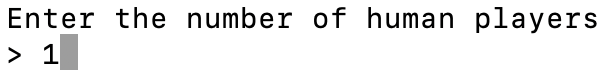
\includegraphics[width=8cm]{./images/human-players-village-war-game.png}
    \caption{Picking the number of human players}
    \label{human-players-village-war-game}
\end{figure}

Starting the game the player is asked to input the number of
human players.

\begin{figure}[H]
    \centering
    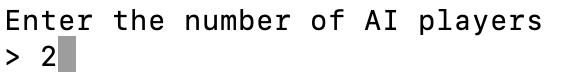
\includegraphics[width=8cm]{./images/ai-players-village-war-game.png}
    \caption{Picking the number of AI players}
    \label{ai-players-village-war-game}
\end{figure}

Then the player is asked to input the number of AI players.

\begin{figure}[H]
    \centering
    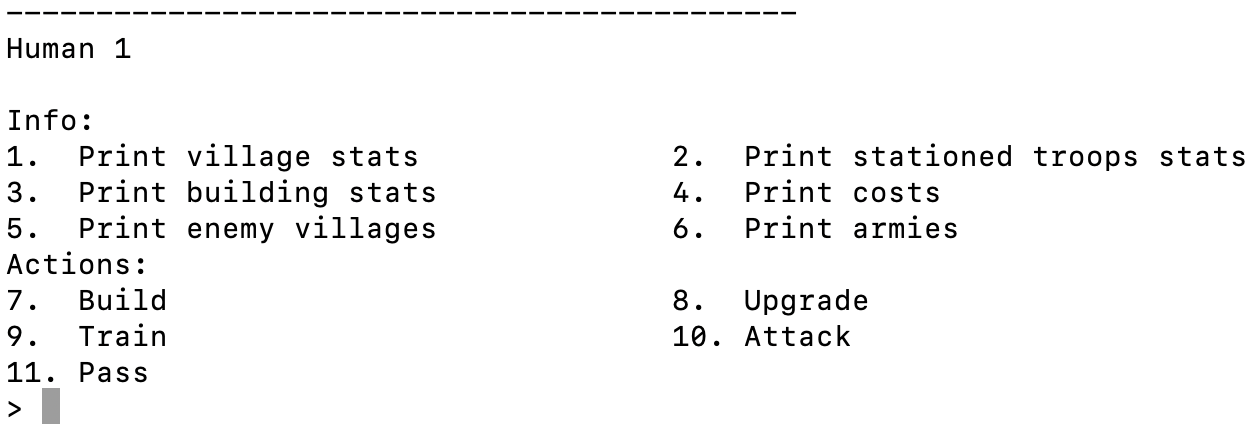
\includegraphics[width=12cm]{./images/player-menu-village-war-game.png}
    \caption{Menu for the human players}
    \label{player-menu-village-war-game}
\end{figure}

The game loop will start. Each human player will be prompted
with a menu of options. There are two categories: \textbf{Info}
and \textbf{Actions}.

The \textbf{Info} category contains options which provide the
player with information about his own village, enemy villages,
armies and costs. Every option in the \textbf{Info} category is
self--explanatory.

The \textbf{Actions} category contains options which affect the
state of the game such as \textit{building}, \textit{training}
and \textit{attacking}. Finally, the player can decided to pass
the turn to the next player.

All players by default will start with $50$ ``food'', ``metal''
and ``mana''. The player can use these resources to build
or upgrade buildings and train troops.

The following types of building can be built:

\begin{enumerate}
    \item Academy (to generate wizards)
    \item Foundation (to generate scouts)
    \item Arena (to generate brawlers)
    \item Farm (to generate food)
    \item Mine (to generate metal)
    \item Mana Tower (to generate mana)
\end{enumerate}

As described in the above list there are three types of troops:

\begin{enumerate}
    \item Wizard (high attack, low health, medium speed, low
        carrying capacity)
    \item Brawler (high attack, high health, slow speed, medium
        carrying capacity)
    \item Scout (medium attack, medium health, high speed, high
        carrying capacity)
\end{enumerate}

\subsubsection*{\ul{Building}}

\begin{figure}[H]
    \centering
    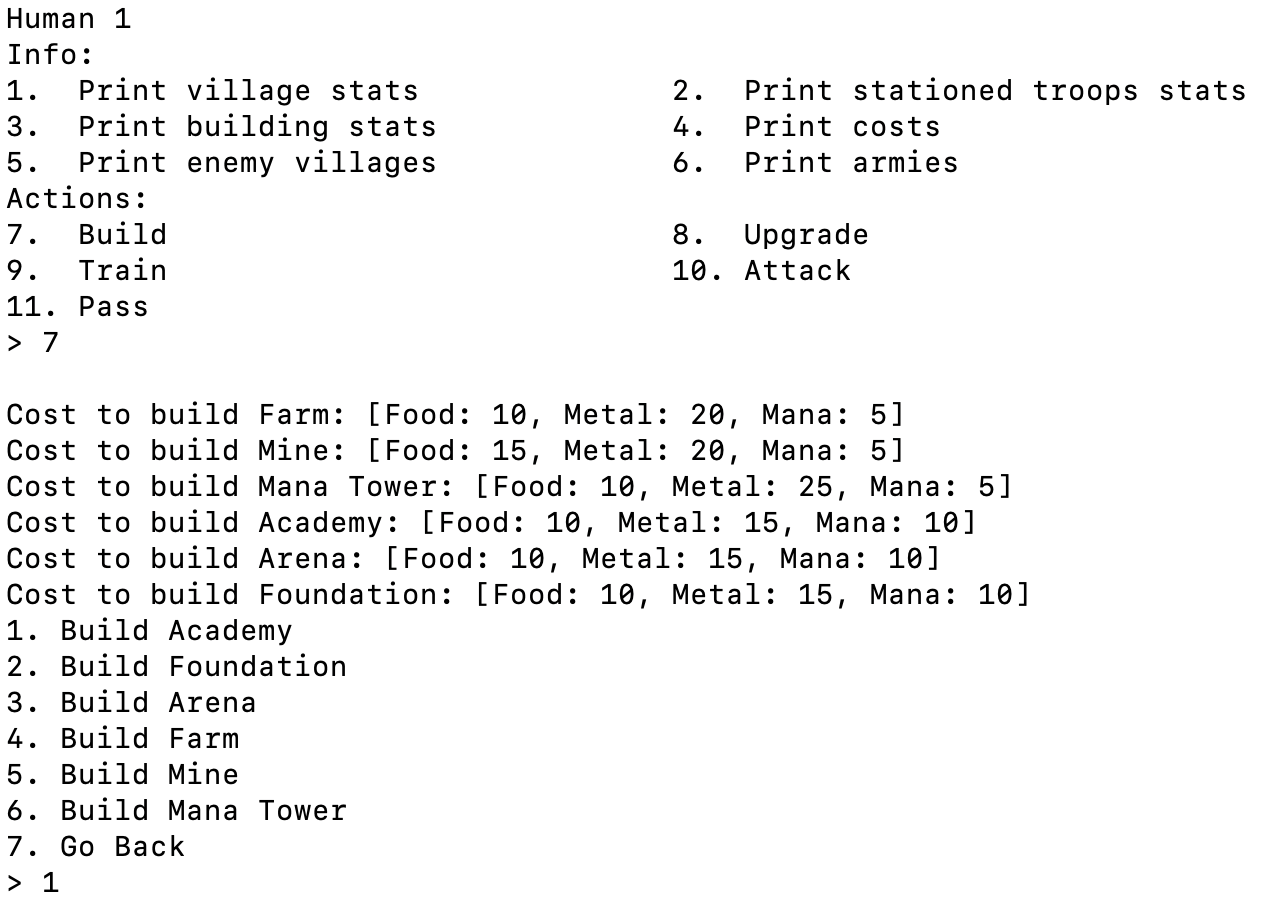
\includegraphics[width=12cm]{./images/building-village-war-game.png}
    \caption{Building an Academy in the player's village}
    \label{building-village-war-game}
\end{figure}

As depicted above in figure \ref{building-village-war-game}, the
player is prompted with the different costs of the different
buildings. If the player does not have enough resources for
building he/she is notified.

\begin{figure}[H]
    \centering
    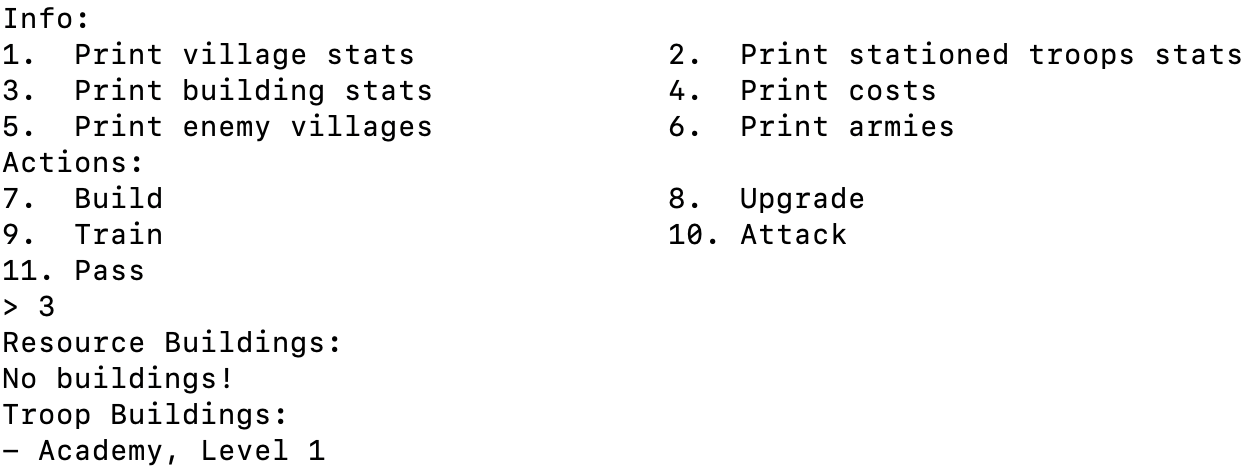
\includegraphics[width=12cm]{./images/buildings-info-village-war-game.png}
    \caption{Info about buildings in the player's village}
    \label{buildings-info-village-war-game}
\end{figure}

As shown in figure \ref{buildings-info-village-war-game}, the
buildings can have different levels of productivity. The initial
level of productivity for all buildings is $1$.

\subsubsection*{\ul{Upgrading}}

\begin{figure}[H]
    \centering
    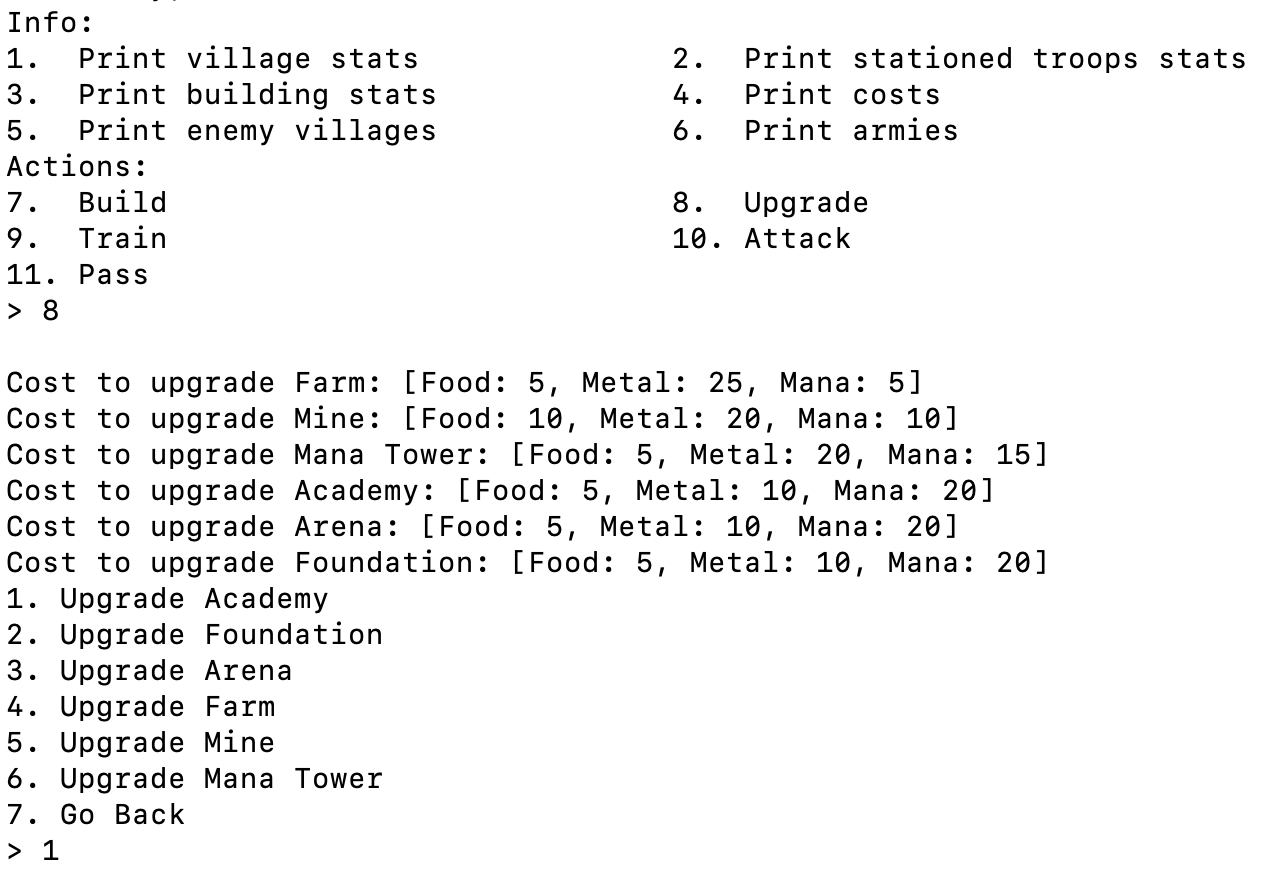
\includegraphics[width=12cm]{./images/upgrading-village-war-game.png}
    \caption{Upgrading an Academy in the player's village}
    \label{buildings-info-village-war-game}
\end{figure}

Upgrading the building increases the building's level of
productivity. This has the effect of generating more resources
or troops per round.  Similarly, if the player does not have
enough resources for upgrading he/she is notified. 

Additionally, the building which is upgraded first is the oldest
building.

\subsubsection*{\ul{Training}}

\begin{figure}[H]
    \centering
    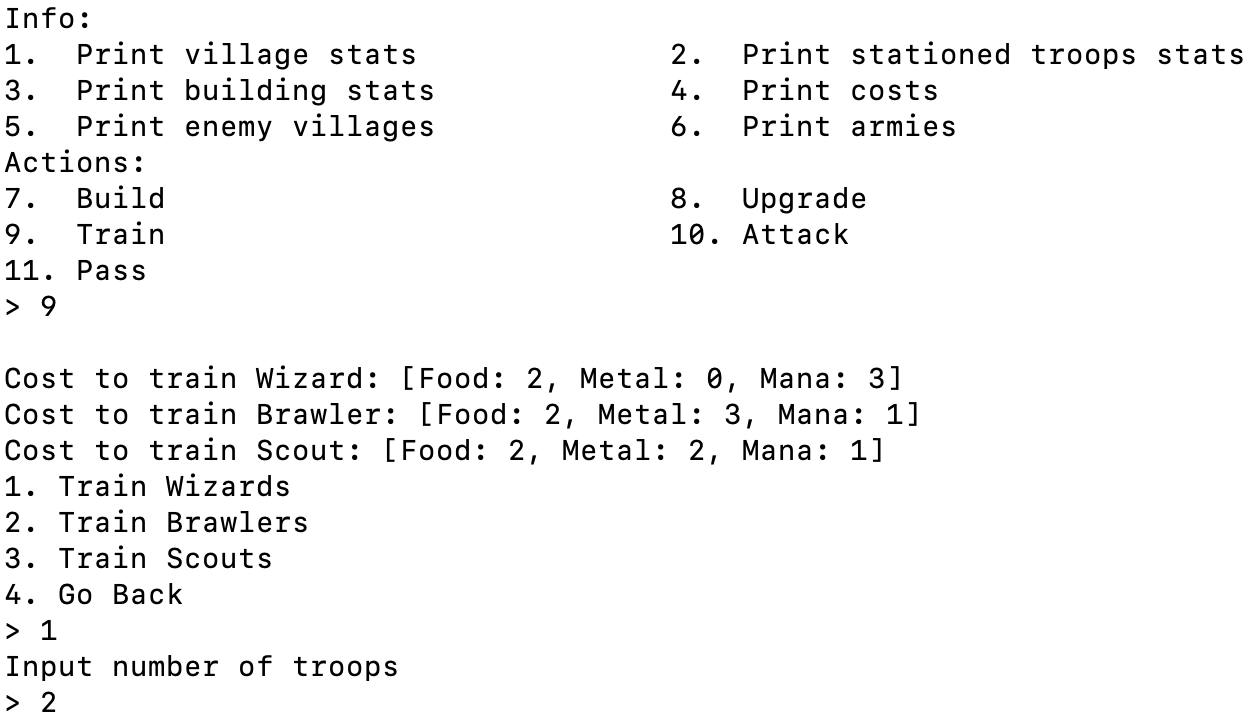
\includegraphics[width=12cm]{./images/training-village-war-game.png}
    \caption{Training Wizards in the player's village}
    \label{buildings-info-village-war-game}
\end{figure}

Training troops increases the overall stats of the chosen
troops. Similarly if the player does not have enough resources
or troops he/she is notified.

Additionally, the training scheme is the same as for buildings
i.e. the oldest troops are trained first, and each troop has an
initial level of $1$ and a maximum level of $3$.

\subsubsection*{\ul{Attacking}}

\begin{figure}[H]
    \centering
    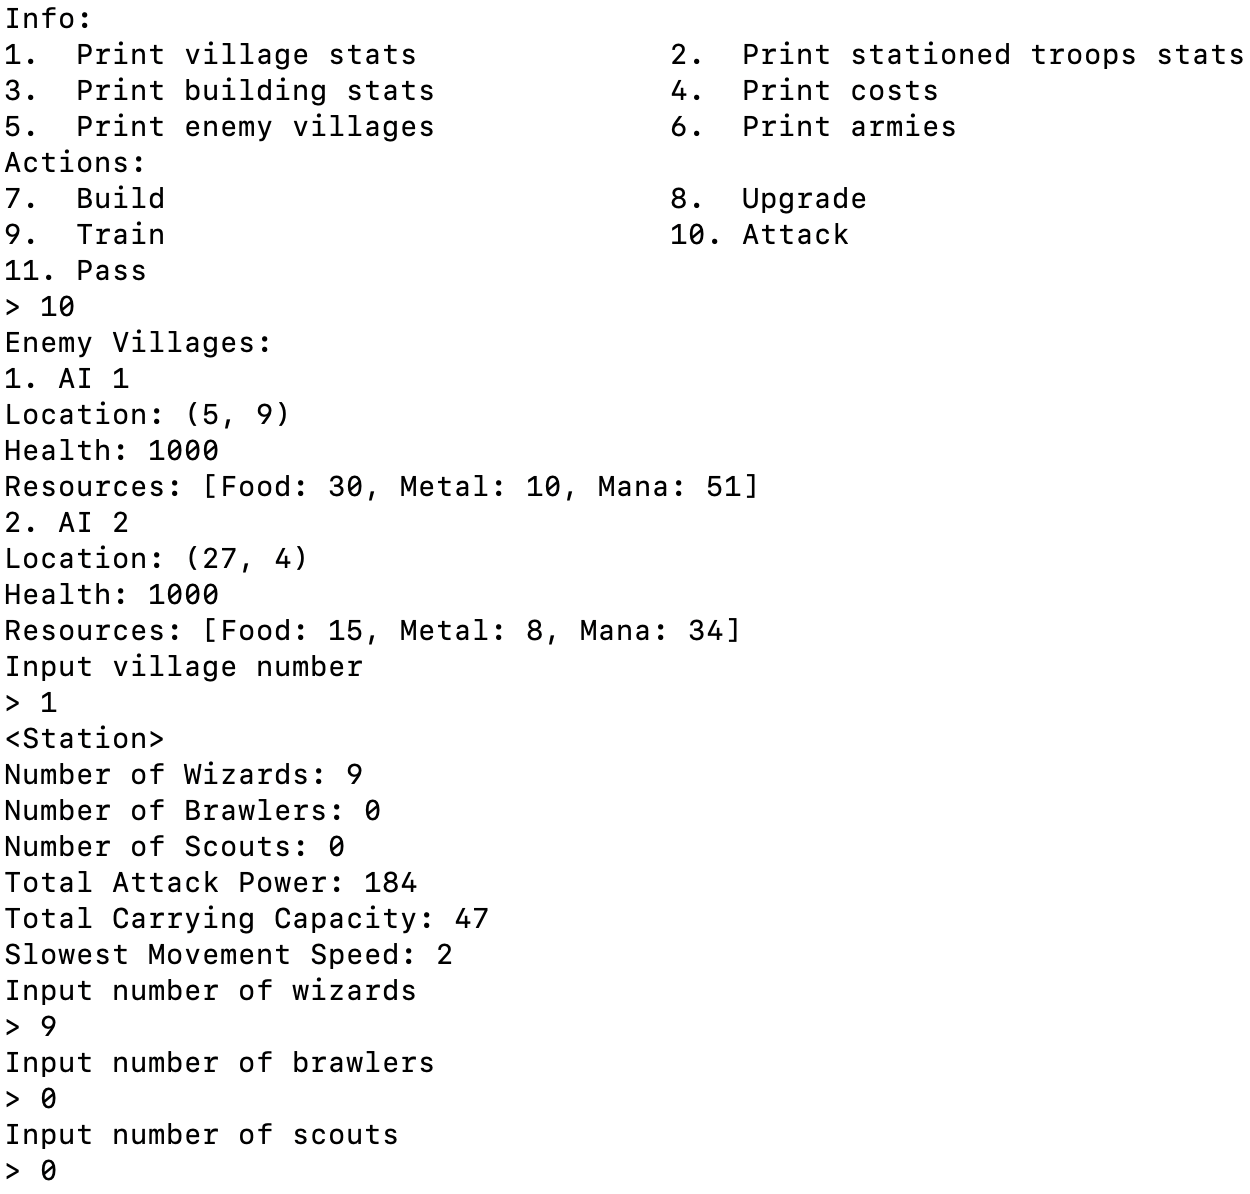
\includegraphics[width=12cm]{./images/attacking-village-war-game.png}
    \caption{Attacking another village with Wizards in the player's village}
    \label{attacking-village-war-game}
\end{figure}

To attack another village the player needs to pick a enemy
village to attack. Then the player must specify the composition
of the army.

Again if the player does not have enough troops he/she is
notified.

The troops will be moved from the village station into the army.
This means that the village will have less defensive power
making it more vulnerable to attack.

\begin{figure}[H]
    \centering
    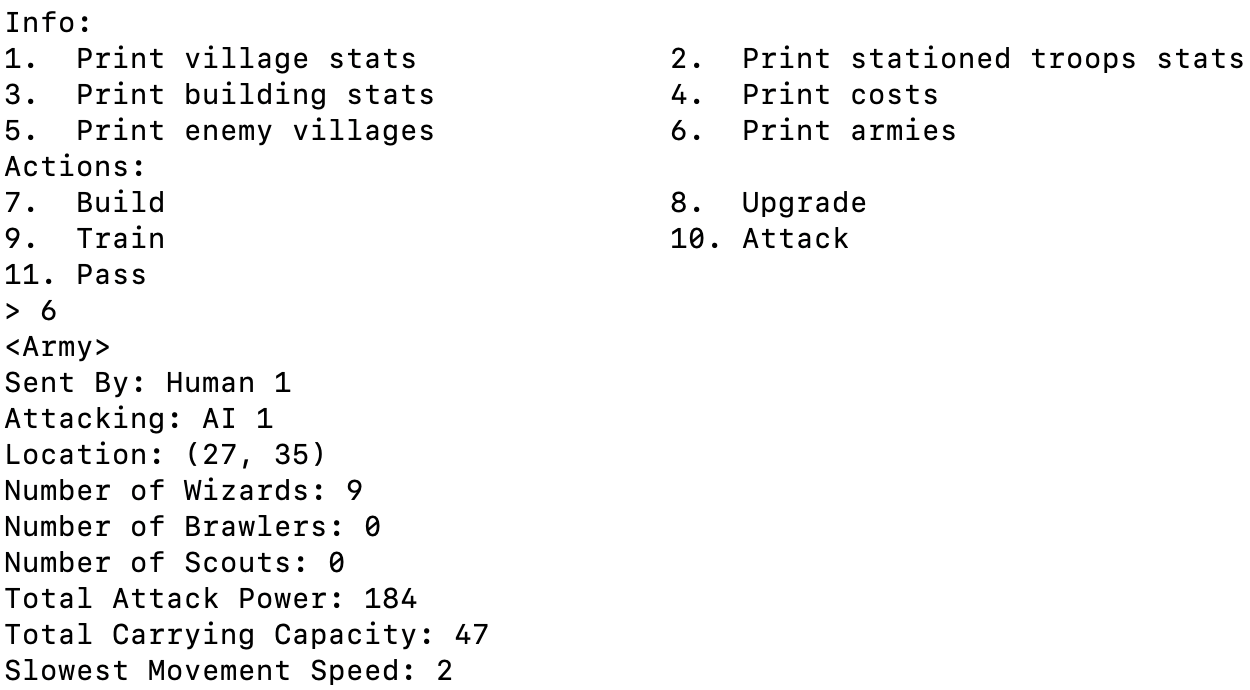
\includegraphics[width=12cm]{./images/armies-info-village-war-game.png}
    \caption{Viewing an army marching towards an enemy village}
\end{figure}

Additionally, when the army arrives at it destination the player
will be notified of whether the attack was successful or
unsuccessful.

\subsubsection*{\ul{Incorrect Player Input}}

In all instances where the player input is unexpected or
incorrect, the player is notified. All error messages are
handled in the \texttt{HumanPlayer} class. 

Moreover, error handling was performed by returning a
\texttt{Status} enum which contains a number of possible errors
which the program might encounter.

\textbf{Note:} Exceptions were avoided at all costs as they
obscure control flow. Moreover, most errors do not arise
because of exceptional circumstances. Exceptions were handled
only when thrown from the standard library.

\subsubsection*{\ul{Quitting}}

Any human player can quit by pressing Ctrl-C.

\subsection{Design}

\begin{figure}[H]
    \centering
    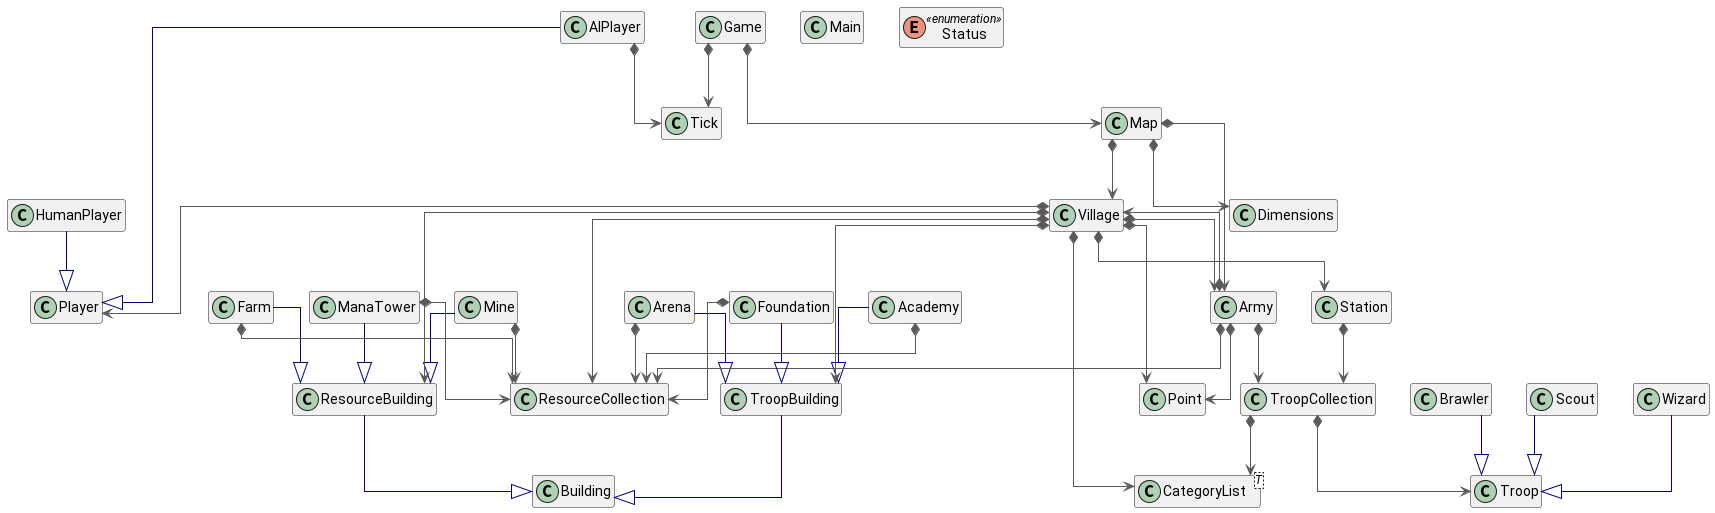
\includegraphics[width=17cm]{./village-war-game-uml/village-war-game.png}
    \caption{A UML diagram (without members) of the game}
\end{figure}

\textbf{Note:} The full class diagrams will not be displayed as
they would consume to many pages.

In terms of design the specification was followed closely.

\subsubsection{The Game Class}

The Game class is essentially the entry point to our program.
The main method will create a new instance of the Game class and
it will call the \texttt{run()} method to start the game. The
Game class houses a Map and has two main phases, the setup
phase and the game loop phase. The setup phase essentially
creates all the objects and which are required at the start.

\textbf{Note:} The size of the Map varies depending on the
number of players. Moreover, it tries to spread out all the
villages evenly on the map to ensure that no villages are to
close to each other.

The game loop phases is essentially, where all the game play
start and operations which need to occur everything every round
of the game are done. Also, every round the game tick is
increased. This allows us to keep track and try to quantify at
what stage the game is.

\subsubsection{Map \& Village Design}

The Map class will only contain two lists. These are a list of
villages and a list of armies. This approach instead or actually
storing everything in a 2D array has a couple of benefits.
Firstly, this makes dealing with objects a lot easier since
there is no need to move objects from one location in
to another in the array. Also, it is easier and more efficient to
just store the location of the entity directly with the entity.
This means that getting the location of an entity is fast.
Moreover, it also means that you can have multiple objects which
occupy the same location without interfering with each other.
This is obviously useful since we do not have to worry about
intersecting armies.

The Village of each player is essentially the hub where all
actions are performed. This also unfortunately means that the
village has to be polluted with a lot of action methods. This is
only the case due to the limitations present in Java's generics
and reflection capabilities.

\textbf{Note:} This is ideally circumvented by actually,
dropping all OOP design and instead using singular entities
like: Troop and Building, then providing a builder which
constructs Troops and Buildings with specific statics and
identifiers remove the need for reflection and generics to deal
will all types of troops and buildings, whilst retaining the
possibility of quickly extending the types of troops and
buildings very easily.

\subsubsection{Player Design}

For the player, there is a main abstract class and two
subclasses which implement the interface defined in the abstract
class. The two subclasses are AIPlayer and HumanPlayer. Then
each Village has a Player field which we can populate with a
player. Since both types of players have the same interface and
they can interact with the village in the same way. Also it
makes swapping between an AI player and human player easy.

\textbf{Note:} A simple reference to the Tick object present in
the game object is also present in all AI players. This can
allow for more complicated AI behaviour because it allows for
the artificial creation of game stages similar to chess for
example: the opening, mid-game and the end-game.

\subsubsection{Resource Design}

In particular in terms implementation since  we need a
substantial amount of resources to almost anything in the game
it simply does not make sense to create a Resource class and
then subclasses of specific types of resources. The issue with
doing this is that handling the resources would have been very
difficult. Additionally, it would have required the continuous
creation of resources which would have definitely taken time
since allocating memory is an expensive operation. Also as
objects they would have carried no internal state what so ever
and only the presence of that type of which add to the
cumulative sum of resources makes has meaning. Hence, everything
was design around having one ResourceCollection which holds
counters of the amount of resources of all the different types.

This substantially improves performance since there is no need
for a lot of allocations and it means that overall handling
resources is less cumbersome.

\subsubsection{Troop Design}

Again there is a Troop abstract class which which specifies the
behaviour of all troops and then there are subclasses which
initialize their fields with specific values according to the
strength and weaknesses each Troop type (as described above in
the player guide.)

Further more an important data structure built on top of the
CategoryList is the TroopCollection. This class facilitates the
grouping of all troops even of different class types into one
object. This object is able to send and receive troops,
calculate the total attack power etc.

Additionally, we have to other classes which compose a
TroopCollection. These are Army and Station. The Army as the
name implies is able to roam the map whilst the Station is part
of the village.

The difference between these two is that the Army is able to
move and exist separately of the village. Additionally, it has a
lot of extra methods which facilitate combat with a village.

\subsubsection{Building Design}

This is the biggest inheritance hierarchy. There is a main
abstract class called Building and two abstract subclasses which
are TroopBuilding and ResourceBuilding which differentiate
between troop generating buildings and resource generating
buildings. Initially, the reason for the split was done under
the assumption that the troop buildings require an additional
method to train troops. However, this was no longer needed later
on in development. However, changing would have resulted in
changing quite a few parts of the code to deal with a single
level of inheritance. So, this system was kept. Since training
is not actually done by the building but by a method in the
troop, to follow game specifications a check to ensure that at
building of the appropriate type exists was put in place.

Moreover, the Village class contains two category lists of type
TroopBuilding and type ResourceBuilding because the CategoryList
class is not powerful enough provide a mechanism where you can
group any collection of objects by the respective category even
if it may be a super class. Also using such a data structure is
either guaranteed to be slow due to requirement of iteration or
memory hungry requiring separate list for all the classes in
the inheritance hierarchy to accommodate searching with any
possible class in the hierarchy.


\subsection{Technical Aspects}

In general, give the above design which is very technical it
meant that most of the coding was simply routine coding with
nothing out of the ordinary. The only notable mentions is the
extensive use of design patterns specifically the builder, the
singleton and the observer and the CategoryList.


\begin{lstlisting}[language=Java, caption={Builder pattern used
for the ResourceCollection}]
public static class Builder {
    private int _food = 0;
    private int _metal = 0;
    private int _mana = 0;
    
    public ResourceCollection build() {
        return new ResourceCollection(_food, _metal, _mana);
    }
    
    public Builder setFood(int food) {
        if (food >= 0) {
            _food = food;
        }
    
        return this;
    }
    
    public Builder setMetal(int metal) {
        if (metal >= 0) {
            _metal = metal;
        }
    
        return this;
    }
    
    public Builder setMana(int mana) {
        if (mana >= 0) {
            _mana = mana;
        }
    
        return this;
    }
}
\end{lstlisting}

As we can see the above code is implementing the builder
pattern. This was helpful because it allowed for the easier
creation of resource collection as sometimes they are also used
to denote cost for example upgrading a building.

\begin{lstlisting}[language=Java, caption={The game Tick class
is a singleton}]
public class Tick {
    private static Tick _instance = null;

    private BigInteger _tick = BigInteger.ZERO;
    private Tick() {}

    public static Tick getInstance() {
        if (_instance == null) {
            _instance = new Tick();
        }

        return _instance;
    }

    // ...
}
\end{lstlisting}

Again similarly, this was useful to ensure that one can use the
Tick object where ever it useful and ensure that there is only
one instance per game.

\begin{lstlisting}[language=Java, caption={The Player class
(contains the notify for the observer pattern)}]
public abstract class Player {
    private final String _name;
    public Player(String name) {
        _name = name;
    }
    public String getName() {
        return _name;
    }
    public abstract void actions(Village village);
    public abstract void notify(String text);
}
\end{lstlisting}

\begin{lstlisting}[language=Java, caption={\texttt{notify()}
being used to notify the player that a army has been defeated in
Village.java}]
public Village enemyTroopArrival() {
    List<Army> clonedArmies = new LinkedList<>(_armies);
    
    for (var army : clonedArmies) {
        if (army.isEnemy(this) && army.arrived()) {
            if (isDestroyed()) {
                army.goBack();
            } else {
                if (!army.attack().isSuccessful()) {
                    army.getSender().getPlayer().notify("The below army has been defeated\n" + army);
                    _armies.remove(army);
                }
            }
        }
    }
    
    return this;
}
\end{lstlisting}

The observer pattern is used because it is useful for notifying
players of events in game. Specifically, it is used when armies
are defeated or when they arrive back. This helps the player
gain useful information which he/she wouldn't have since the
player's village will never actually interact with the defeated
army again.

\subsection{Testing}

So, there are three types of failures which our application has
to cater for:

\begin{enumerate}
    \item Incorrect input i.e. failure to parse input into
        correct type.
    \item Failure due to invalid option or out of bounds e.g.
        option $12$ does not exist.
    \item Failure due to insufficient resources or troops.
\end{enumerate}

% add images for all three types of errors

Each input was manually tested to ensure that it is not possible
to plunge the game into an invalid where behaviour is not
properly defined.


% along with a image demonstrating the behaviour to make sure
% that certain features are working

Additionally, the game was further manually tested in a form of
white-box testing to ensure that the game behaviour is as
expected.

\subsection{Limitations \& Improvements}

\ul{Limitation:} The user interface is very hard to navigate
around and not intuitive. Additionally, crucial information for
the player to play strategically, is hidden behind info options
which is decision taken to reduce screen clutter.

\ul{Solution:} Creating a GUI which the user can use would make
the overall experience of playing the game better. This is
because the user interface can be better to provide the user
with important information quickly and easily accessible
actions.

\ul{Limitation:} Dealing with different object types which all
have identical features just different values is not ideal. This
is because it increases complexity due to the restrictions of
the type checking in a language. To circumvent this issue
facilities such as generics and reflection are used. However, in
Java these are not really first-class features with the same
power as in other languages.

\ul{Solution:} Settling on a simpler entity system where
inheritance is a avoided as much as possible reduces issues
related type checking enforced by the compiler and hence there
is no need for dealing with generics or reflection making the
overall code significantly simpler.

\ul{Limitation:} The amount of options and choices the user can
make is limited. This is mainly due to the how clunky the user
interface it.

\ul{Solution:} Changing to GUI can allow the application to grow
in terms of complexity

\section{Minesweeper}

\subsection{Language Choice}

\cpp{} was chosen for Minesweeper because it has a fixed board
size of $16 \times 16$. This means that it is possible to stack
allocate every object removing the need for dynamic memory
allocation. This is facilitated by \texttt{std::array} from the
Standard Template Library (STL) which allows for the creation of
fixed size arrays on the stack.

\subsection{User Guide}

\subsubsection{Download, Compiling \& Running}

\begin{enumerate}
\item
    Clone the repository.
\begin{lstlisting}
$ git clone https://github.com/JuanScerriE/minesweeper
\end{lstlisting}

\item
    Compile the tests and the game.

    \textbf{Note:} Make sure that \texttt{gtest} and
    \texttt{ncurses} are installed for the tests and the game,
    respectively.
\begin{lstlisting}
$ cd minesweeper ; ./compile.sh
\end{lstlisting}

\item
    Run the tests.

    \textbf{Note:} Some tests might fail. This is because the
    implementation of \texttt{srand} and \texttt{rand} differ
    between platforms (specifically macOS and Linux).
\begin{lstlisting}
minesweeper $ ./tests.sh
\end{lstlisting}

\item
    Run the game.
\begin{lstlisting}
minesweeper $ ./run.sh
\end{lstlisting}

\end{enumerate}

\subsubsection{Playing}

\begin{figure}[H]
    \centering
    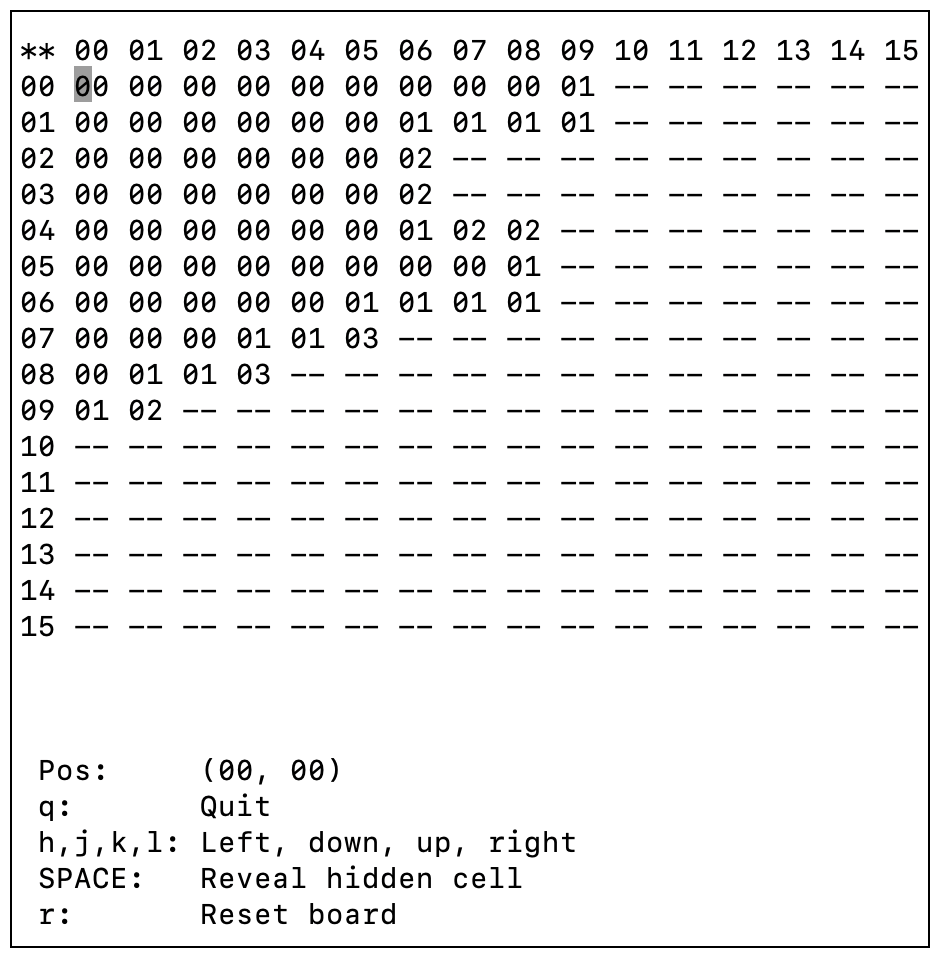
\includegraphics[width=10cm]{./images/playing-minesweeper.png}
    \caption{Playing Minesweeper}
    \label{playing-minesweeper}
\end{figure}

The general guide to playing Minesweeper is described above in
figure \ref{playing-minesweeper}.

\textbf{Note:} \texttt{vim} motions are used to move the cursor.

\begin{figure}[H]
    \centering
    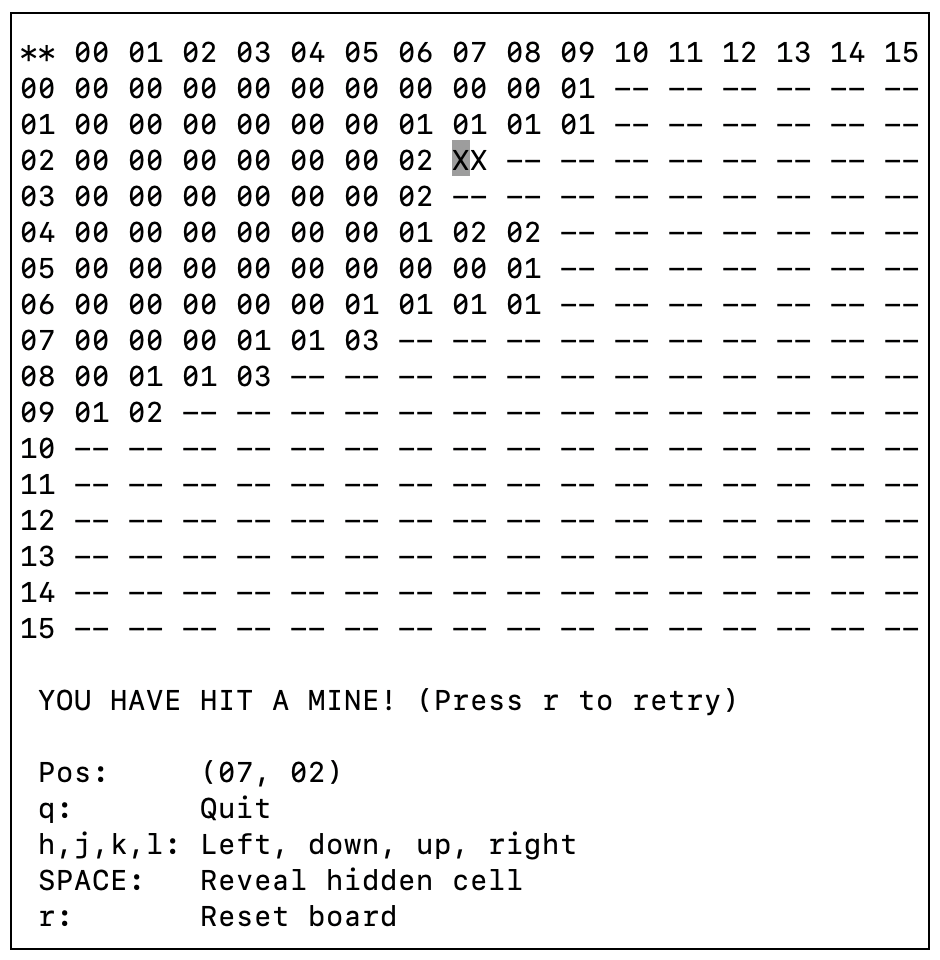
\includegraphics[width=10cm]{./images/hitting-mine-minesweeper.png}
    \caption{Hitting a mine}
    \label{hitting-mine-minesweeper}
\end{figure}

If the player hits a mine the above message as in figure
\ref{hitting-mine-minesweeper} will be displayed.

\begin{figure}[H]
    \centering
    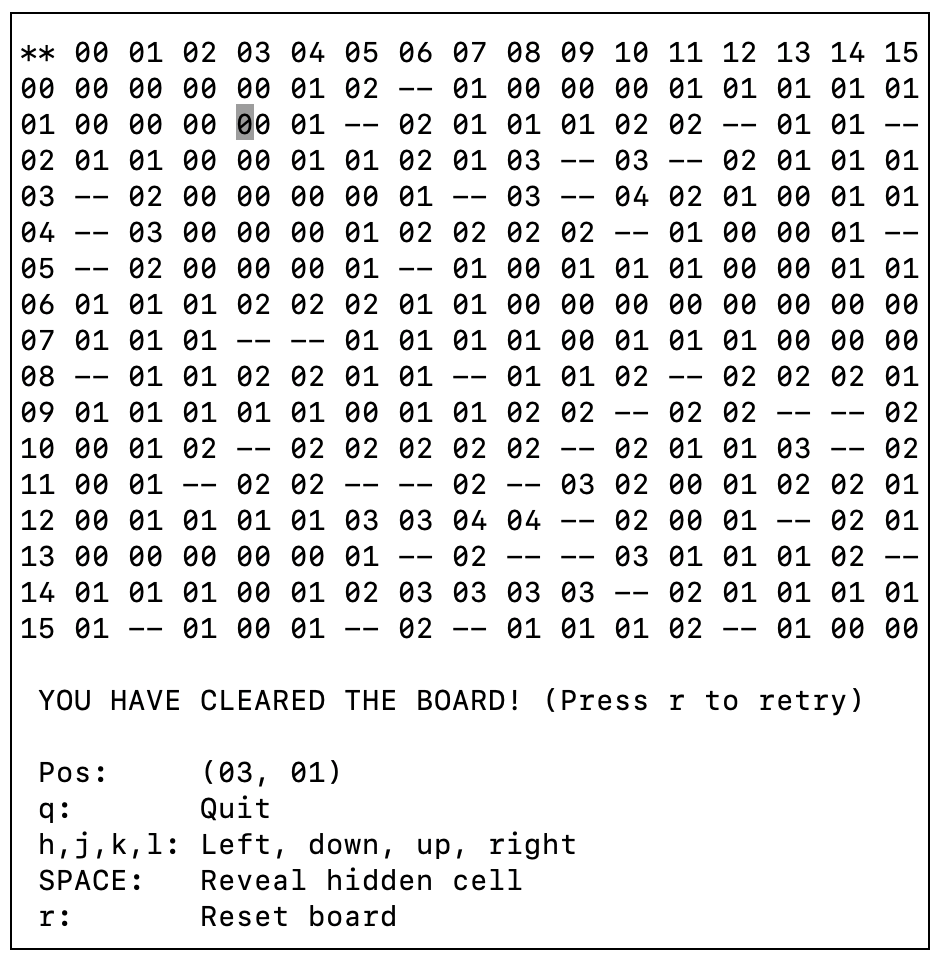
\includegraphics[width=10cm]{./images/finishing-minesweeper.png}
    \caption{Finishing a game of Minesweeper}
    \label{finishing-minesweeper}
\end{figure}

If the player manages to clear all the cells without hitting a
mine the above message as in figure \ref{finishing-minesweeper}
will be displayed.

Finally, there is an additional \textit{secret} command to
automatically complete the board without hitting a mine. The
user needs to press \texttt{W} (\texttt{shift + w}).

\textbf{Note:} This only works if the user has at least revealed
one cell. This is because the board is populated with all the
mines after the first reveal to ensure a player never hits a
mine on his first try.

\subsection{Design}

\begin{figure}[H]
    \centering
    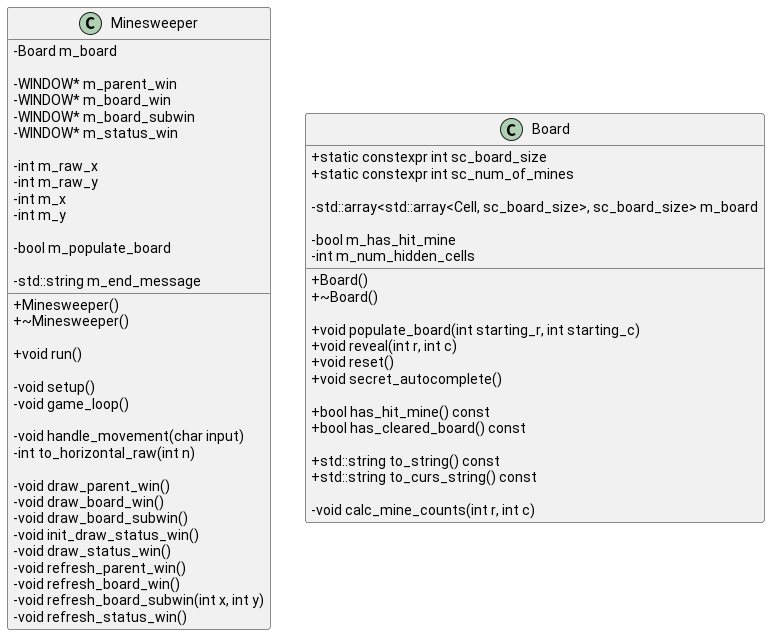
\includegraphics[width=17cm]{minesweeper-uml/minesweeper-and-board.png}
    \caption{Class diagrams of the Minesweeper class and the Board class}
\end{figure}

\begin{figure}[H]
    \centering
    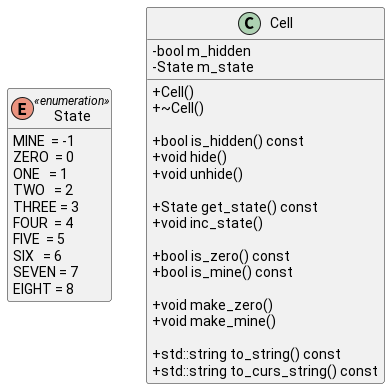
\includegraphics{minesweeper-uml/cell.png}
    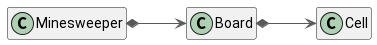
\includegraphics{minesweeper-uml/relations.png}
    \caption{A class diagram of the Cell class State enum and a
    UML diagram (without members) of the game}
\end{figure}

The Minesweeper class contains the user interface code, that
is it contains all \texttt{ncurses} specific code. The class
also handles user input.

The Board class contains the majority of the game logic. It is a
part of the Minesweeper class, that is if a Minesweeper object
ceases to exist so does the Board object. Further more the
actual board \texttt{m\_board} is a grid of Cell objects. Also
the lifetime of the objects is managed by the Board since when
the board ceases to exist so do the cells.

\subsection{Testing}

\begin{figure}[H]
    \centering
    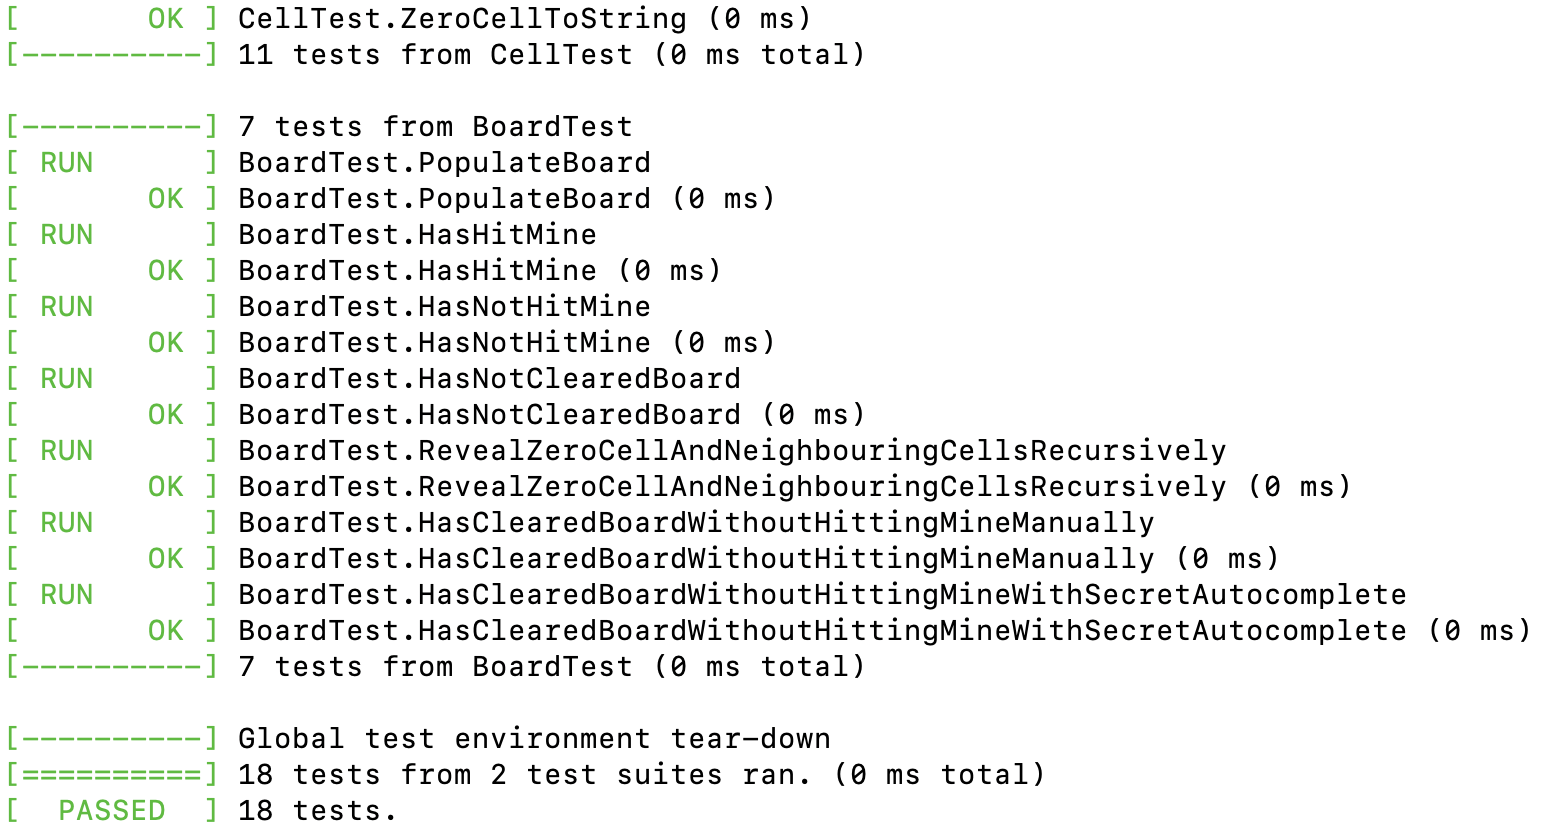
\includegraphics[width=10cm]{./images/unit-tests-minesweeper.png}
    \caption{Unit tests for Minesweeper (on macOS Ventura 13.1)}
\end{figure}

Black-box Testing and Unit Testing were used to test the
application. For unit testing \texttt{gtest} is required.

\begin{figure}[H]
    \centering
    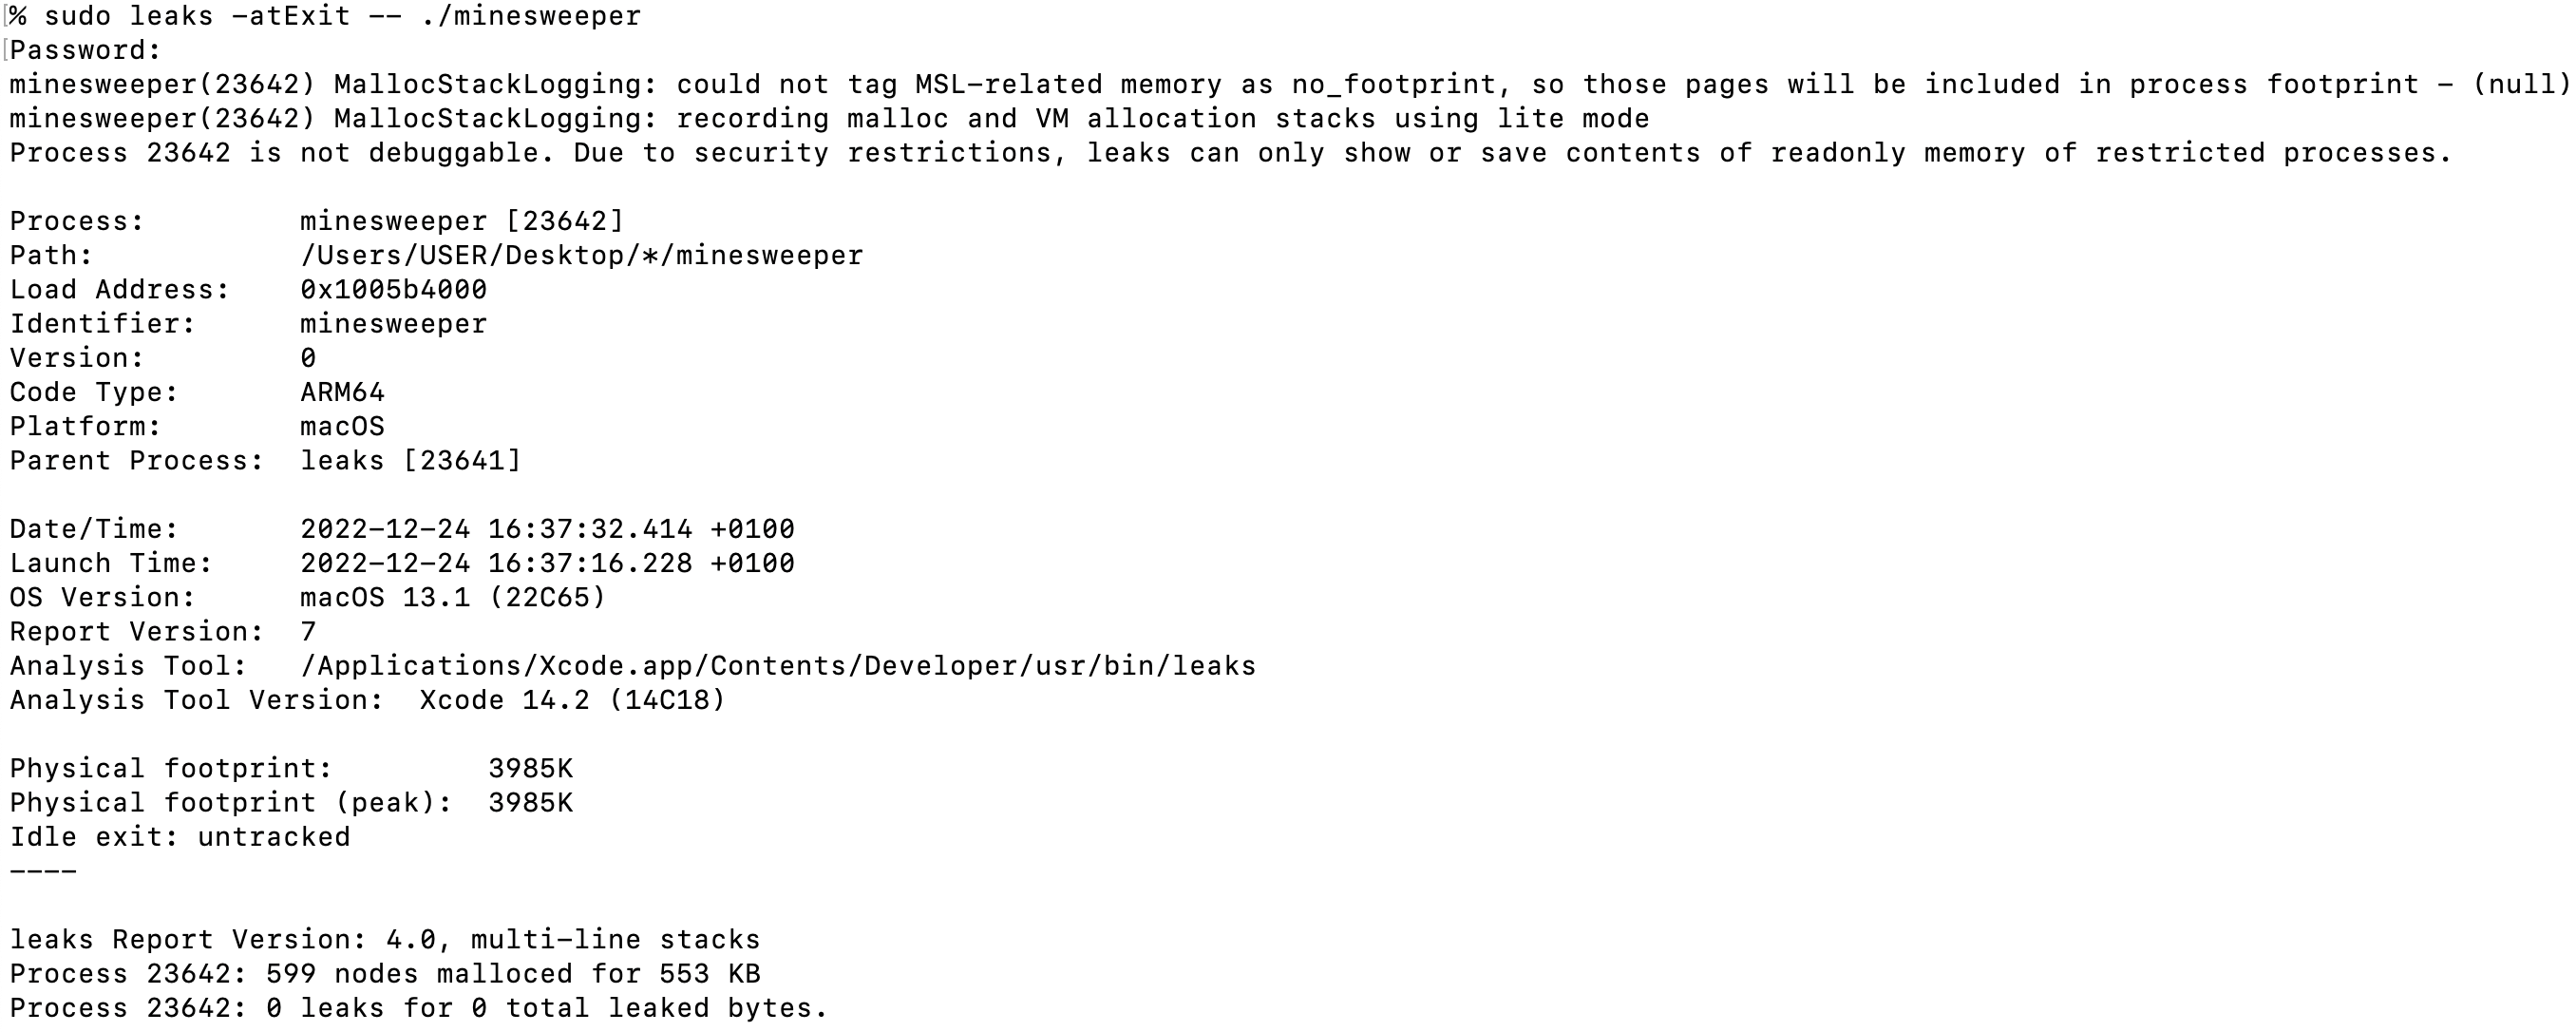
\includegraphics[width=14cm]{./images/leaks-minesweeper.png}
    \caption{Testing for memory leaks (on macOS Ventura 13.1)}
\end{figure}

Furthermore, to test for memory leaks, on macOS, \texttt{leaks}
was used and, on Linux, \texttt{valgrind} was used.
\texttt{leaks} reported not memory leaks whilst
\texttt{valgrind} reported leaks from \texttt{ncurses}.

\subsection{Limitations \& Improvements}

\ul{Limitation:} The unit tests are not cross-platform; four of
the unit tests fail on Linux. This is mostly due to differing
implementations of \texttt{srand()} and \texttt{rand()} on
different platforms.

\ul{Solution:} Create a custom random number generated. This
guarantees the same result across different platforms.

\ul{Limitation:} The \texttt{ncurses} library leaks memory on
Linux whilst on macOS it does not.

\ul{Solution:} This seems to be intended behaviour from
\texttt{ncurses}. Read the man page at
\url{https://man7.org/linux/man-pages/man3/curs_memleaks.3x.html}

\end{document}
